\section{Implementation}
\label{sec:implementation}

This section describes details in both the NDN-IoT framework and Flow application components.

\subsection{NDN-IoT framework}
\label{sec:implementation-ndn-iot}

The NDN-IoT framework is a set of libraries in Python, C++, JS and C\# built on top of the NDN Common Client Libraries.
Each library in the framework implements naming, trust management and rendezvous in Section~\ref{sec:design}, which are organized into three functional blocks: bootstrap, discovery and application-level pub/sub.
The overall structure of the framework is shown in Figure~\ref{fig:ndn-iot-framework-structure}.

\begin{figure}[!t]
\centering
\includegraphics[width=0.95\columnwidth]{ndn-iot-structure.pdf}
\caption{The structure of NDN-IoT framework.}
\label{fig:ndn-iot-framework-structure}
\end{figure}

The rest of this subsection covers each functional block, and an AS implementation available in Python and JavaScript.

% NDN-IoT client libraries
\emph{Bootstrap} follows the suggestion in section VI.B and VI.C of \cite{ndn-iot}, and helps with device and application identity setup. 
Its abstractions include: 
\begin{enumerate}
\item KeyChain setup: given a device identity (and optionally an AS name), construct a KeyChain and set up the default device certificate name for this application instance. 
This KeyChain is later used for signing and verification of all application data.
\item Consumer setup: given an application prefix, the Bootstrap module keeps outstanding interest for the application's trust schema (add example), and updates the local copy whenever a later version is received and verified.\footnote{The application trust schema evolves over time, since new device names may be added and authorized to publish under certain application prefixes}
\item Producer setup: given an application prefix, the Bootstrap module requests authorization from the AS to publish under that prefix following the description in Section~\ref{sec:trust-management}.
If the AS authorizes the request, it adds an entry to the application instance's trust schema to reflect the updated trust relationship, and publishes a new version for all consumers of that instance to fetch.
\end{enumerate}

In practice using the Bootstrap object, the application code to set up a gyroscope data producer on a Raspberry Pi may look like follows.
\begin{minted}
[frame=lines,
framesep=2mm,
baselinestretch=1,
fontsize=\footnotesize,
breaklines
]{python}
from ndn_iot_python import Bootstrap
deviceName = Name("/AliceHome/devices/rpi2")
dataPrefix = Name("/AliceHome/flow1/gyros")
appName = "flow1"
face = Face()
bootstrap = Bootstrap(face)
bootstrap.setupDefaultIdentityAndRoot(deviceName, onSetupComplete, onSetupFailed)

def onSetupComplete(certificateName, keyChain)
  bootstrap.requestProducerAuthorization(dataPrefix, appName, onRequestSuccess, onRequestFailed)

def onSetupFailed(message)
  print(message)
\end{minted}

And in application instance ``flow1'', a trust schema built by the AS may contain the following sections.
\begin{minted}[frame=lines,
framesep=2mm,
baselinestretch=1,
fontsize=\footnotesize,
breaklines
]{text}
trust-anchor 
{
  type "base64"
  base64-string "Bv0DD..."
}
\end{minted}
Trust anchor (AS) certificate is installed to the added device during the onboarding process.
This rule is automatically populated by the AS.

\begin{minted}[frame=lines,
framesep=2mm,
baselinestretch=1,
fontsize=\footnotesize,
breaklines
]{text}
rule 
{
  id "Certs"
  for "data"
  filter 
  {
    type "regex"
    regex "^[^<KEY>]*<KEY><>*<ID-CERT>"
  }
  checker 
  {
    type "customized"
    sig-type "rsa-sha256"
    key-locator 
    {
      type "name"
      name "/AliceHome/devices/gateway/KEY/ksk
-1485314801/ID-CERT"
      relation "equal"
    }
  }
}
\end{minted}
This rule mandates that all certificates should be signed by the gateway.\footnote{In this iteration of Flow, a single level of device certicates are the only certificates involved in the trust relationship in Section~\ref{sec:trust-management}, thus this simplified rule would suffice.}
This rule is automatically populated by the AS.

\begin{minted}[frame=lines,
framesep=2mm,
baselinestretch=1,
fontsize=\footnotesize,
breaklines
]{text}
rule 
{
  id "discovery-data"
  for "data"
  filter 
  {
    type "regex"
    regex "^[^<discovery>]*<discovery><>*"
  }
  checker 
  {
    type "customized"
    sig-type "rsa-sha256"
    key-locator 
    {
      type "name"
      regex "^[^<KEY>]*<KEY><>*<ID-CERT>"
    }
  }
}
\end{minted}
This rule mandates that all discovery data should be signed. 
And the signer's certificate should be verified according to the previous rule.
This rule is automatically populated by the AS, if one component in this instance indicates that it will call Discovery.

\begin{minted}[frame=lines,
framesep=2mm,
baselinestretch=1,
fontsize=\footnotesize,
breaklines
]{text}
rule 
{
  id "/AliceHome/flow1/gyros"
  for "data"
  filter 
  {
    type "name"
    name "/AliceHome/flow1/gyros"
    relation "is-prefix-of"
  }
  checker 
  {
    type "customized"
    sig-type "rsa-sha256"
    key-locator 
    {
      type "name"
      name "/AliceHome/devices/rpi2/KEY/dsk-
1485374576/ID-CERT"
      relation "equal"
    }
  }
}
\end{minted}
This rule mandates that data under application prefix \ndnName{/AliceHome/flow1/gyros} should be signed by device \ndnName{/AliceHome/devices/rpi2}.
This rule is added to the trust schema after the AS approves the publishing request from \ndnName{/AliceHome/devices/rpi2}.

\emph{Discovery} is implemented following the description in Section~\ref{sec:rendezvous}. 
This mechanism differs from the suggested in Section VI.B of \cite{ndn-iot}, in which the device queries the AS for currently active devices.
We use a sync-based mechanism so that the AS does not have to actively maintain a list of devices online.

In practice, after setting up the Bootstrap object, the application may use the following code to include a discovery module.
\begin{minted}[frame=lines,
framesep=2mm,
baselinestretch=1,
fontsize=\footnotesize,
breaklines
]{python}
from ndn_iot_python import Discovery, Observer

class MyObserver(Observer):
  def onDiscovered(name, description):
    print(name.toUri() + description)

keyChain = bootstrap.getKeyChain()
certName = bootstrap.getDefaultCertificateName()
syncPrefix = Name("/AliceHome/discovery/devices")
discovery = Discovery(face, keyChain, certName, syncPrefix, MyObserver())

description = "My Raspberry Pi device"
deviceName = Name("/home/devices/rpi2")
discovery.publishObject(deviceName, description)
\end{minted}

\emph{Application-level pub/sub} follows the suggestion in Section VI.F of \cite{ndn-iot}, and provides the following abstractions:
\begin{enumerate}
\item Consumer for timestamp namespace (/prefix/[timestamp]): this consumer uses oustanding interest with range exclusion to ask for latest piece of data, and upon data retrieval and successful verification, updates the range exclusion with the received timestamp.
\item Consumer for sequence-number namespace (/prefix/[sequence-number]): this consumer pipelines interest for the next few sequence numbers, and upon data retrieval and successful verification, issues an interest for the sequence number after the last one in the pipeline.
\end{enumerate}

In practice, after setting up the Bootstrap object, the application may use the following code to include a sequence number consumer module.

\begin{minted}[frame=lines,
framesep=2mm,
baselinestretch=1,
fontsize=\footnotesize,
breaklines
]{python}
from ndn_iot_python import AppConsumerSequenceNumber
keyChain = bootstrap.getKeyChain()
pipelineSize = 5
consumer = AppConsumerSequenceNumber(face, keyChain, pipelineSize)
prefix = Name("/home/flow1/gyros")
consumer.consume(prefix, onData, onTimeout, onVerifyFailed)
\end{minted}

% AS
\emph{The AS} is implemented based on the team's previous work on NDN-pi (citation: ndn-pi TR).
The framework provides a server implementation in Python, which we run on a Raspberry Pi serving as AS in Flow application.
The AS server implementation updated the codebase to work with PyNDN2 2.0b4, with major updates to security module interface, including using CCL library's built-in public/private key storages.
% \footnote{We now use BasicIdentityStorage and FilePrivateKeyStorage for key storage, and ConfigPolicyManager for data verification, whereas the old implementation, developed at a time when PyNDN security library module was evolving, used custom derived classes (for example, IotPrivateKeyStorage).}

AS clients are available in both Python and JavaScript in order to support application components running on various (Ubuntu, OSX, Raspbian, and browser) platforms.
The JavaScript client uses library's IndexedDb for key storage, and the key storage in browser is origin-based. \footnote{Which means in our installation the webpage that adds this ``device'' and the webpage that publishes application content should be hosted under the same origin.}
Recall that we use a manufacturer given identity to onboard a device, which in browser application's case is not available. 
Instead we generate and store a random string if one doesn't already exist, to use as the manufacturer name of the device currently running the browser.

\subsection{Flow application components}

% Subsystems
In our application prototype, each of the components is implemented as the following:
\begin{enumerate}
\item \emph{Indoor positioning}: We use OpenPTrack,\footnote{\url{http://openptrack.org/about/}} a multi-camera person tracking system.
The NDN producer for OpenPTrack\footnote{\url{https://github.com/OpenPTrack/ndn-opt/}} (written in C++) publishes the position of each person at a 30Hz rate, along with lower rate metadata about active tracks. 
A consumer of track data first fetches the active track IDs contained in the metadata, named in a timestamp namespace, and then uses the IDs to construct interest names to fetch the actual position, named in a sequence number namespace.
The interest and data exchange in this process is shown in Figure~\ref{fig:message-flow-in-flow-installation}, between the visualization component and the indoor positioning components (key 1A and 1B).
\item \emph{Wearable sensing}: We use an RFduino 22301 with gyroscope MPU6050 attached to provide virtual camera control. 
The RFduino follows the pattern for constrained devices described in Section~\ref{sec:constrained-device}, and we introduced a Raspberry Pi as its helper.
The RFduino runs a minimum NDN producer, implemented with the ndn-cpp-lite library\footnote{\url{https://github.com/named-data/ndn-cpp/}}, which generates data at roughly 2Hz rate.
This process of pairing the RFduino and its helper is shown in Fig.~\ref{fig:contrained-devices-bootstrap}.

Message exchanged between the Raspberry Pi helper and the rest of the system is shown in Figure~\ref{fig:message-flow-in-flow-installation}.
\item \emph{Mobile phone interface}: We employ an Android phone that loads a control webpage (written in JavaScript) in a mobile browser to interact with the virtual environment. 
The phone sends out two types of command Interests: the first one matches an OpenPTrack track ID with that of the mobile, and the second one drops an image onto the virtual environment where the user's avatar is standing. 
ID matching is introduced so that the visualization knows the location of the user's avatar (identified by a track ID) when an image drop command Interest is issued by the same user (identified by the mobile's ID).
Keys 2A and 2B in Figure~\ref{fig:message-flow-in-flow-installation} reflects these two types of command interests.
\item \emph{Visualization}: We use the Unity3D\footnote{\url{https://unity3d.com}} game engine for visualization.
The game engine runs C\# NDN data consumers that receive person tracking and virtual camera control data, and a producer that receives image dropping command Interests from the mobile web interface.

A screenshot of the visualization component is also shown in Figure~\ref{fig:message-flow-in-flow-installation}, in which a user has tilted the orientation of the virtual camera, an image is being dropped on his location in the virtual environment, and another user, represented by the small green dot in the distant, is being tracked and rendered on the virtual environment.
\end{enumerate}

\begin{figure}[!t]
\centering
\includegraphics[width=0.95\columnwidth]{constrained-device-authorization.pdf}
\caption{RFduino data publishing with assistance of Raspberry Pi controller}
\label{fig:contrained-devices-bootstrap}
\end{figure}

The implementation for both NDN-IoT framework and Flow application are available online.\footnote{\url{https://github.com/remap/ndn-flow}} 
With documentations dedicated to the framework\footnote{\url{https://github.com/remap/ndn-flow/tree/master/framework}}, its interface\footnote{\url{https://github.com/remap/ndn-flow/tree/master/design/docs}}, installation\footnote{\url{https://github.com/remap/ndn-flow/blob/master/design/DRAFT_FLOW_TechGuide.docx}}, and the application\footnote{\url{https://github.com/remap/ndn-flow/tree/master/application}}.
We installed two instances of the Flow application testbed at UCLA and Huawei. 
Figure~\ref{fig:message-flow-in-flow-installation} shows a summary of our installation at Huawei.\footnote{A screen recording of the running system can be found at \url{https://www.youtube.com/watch?v=MNI_qd75SPQ}}

\begin{figure*}[!t]
\centering
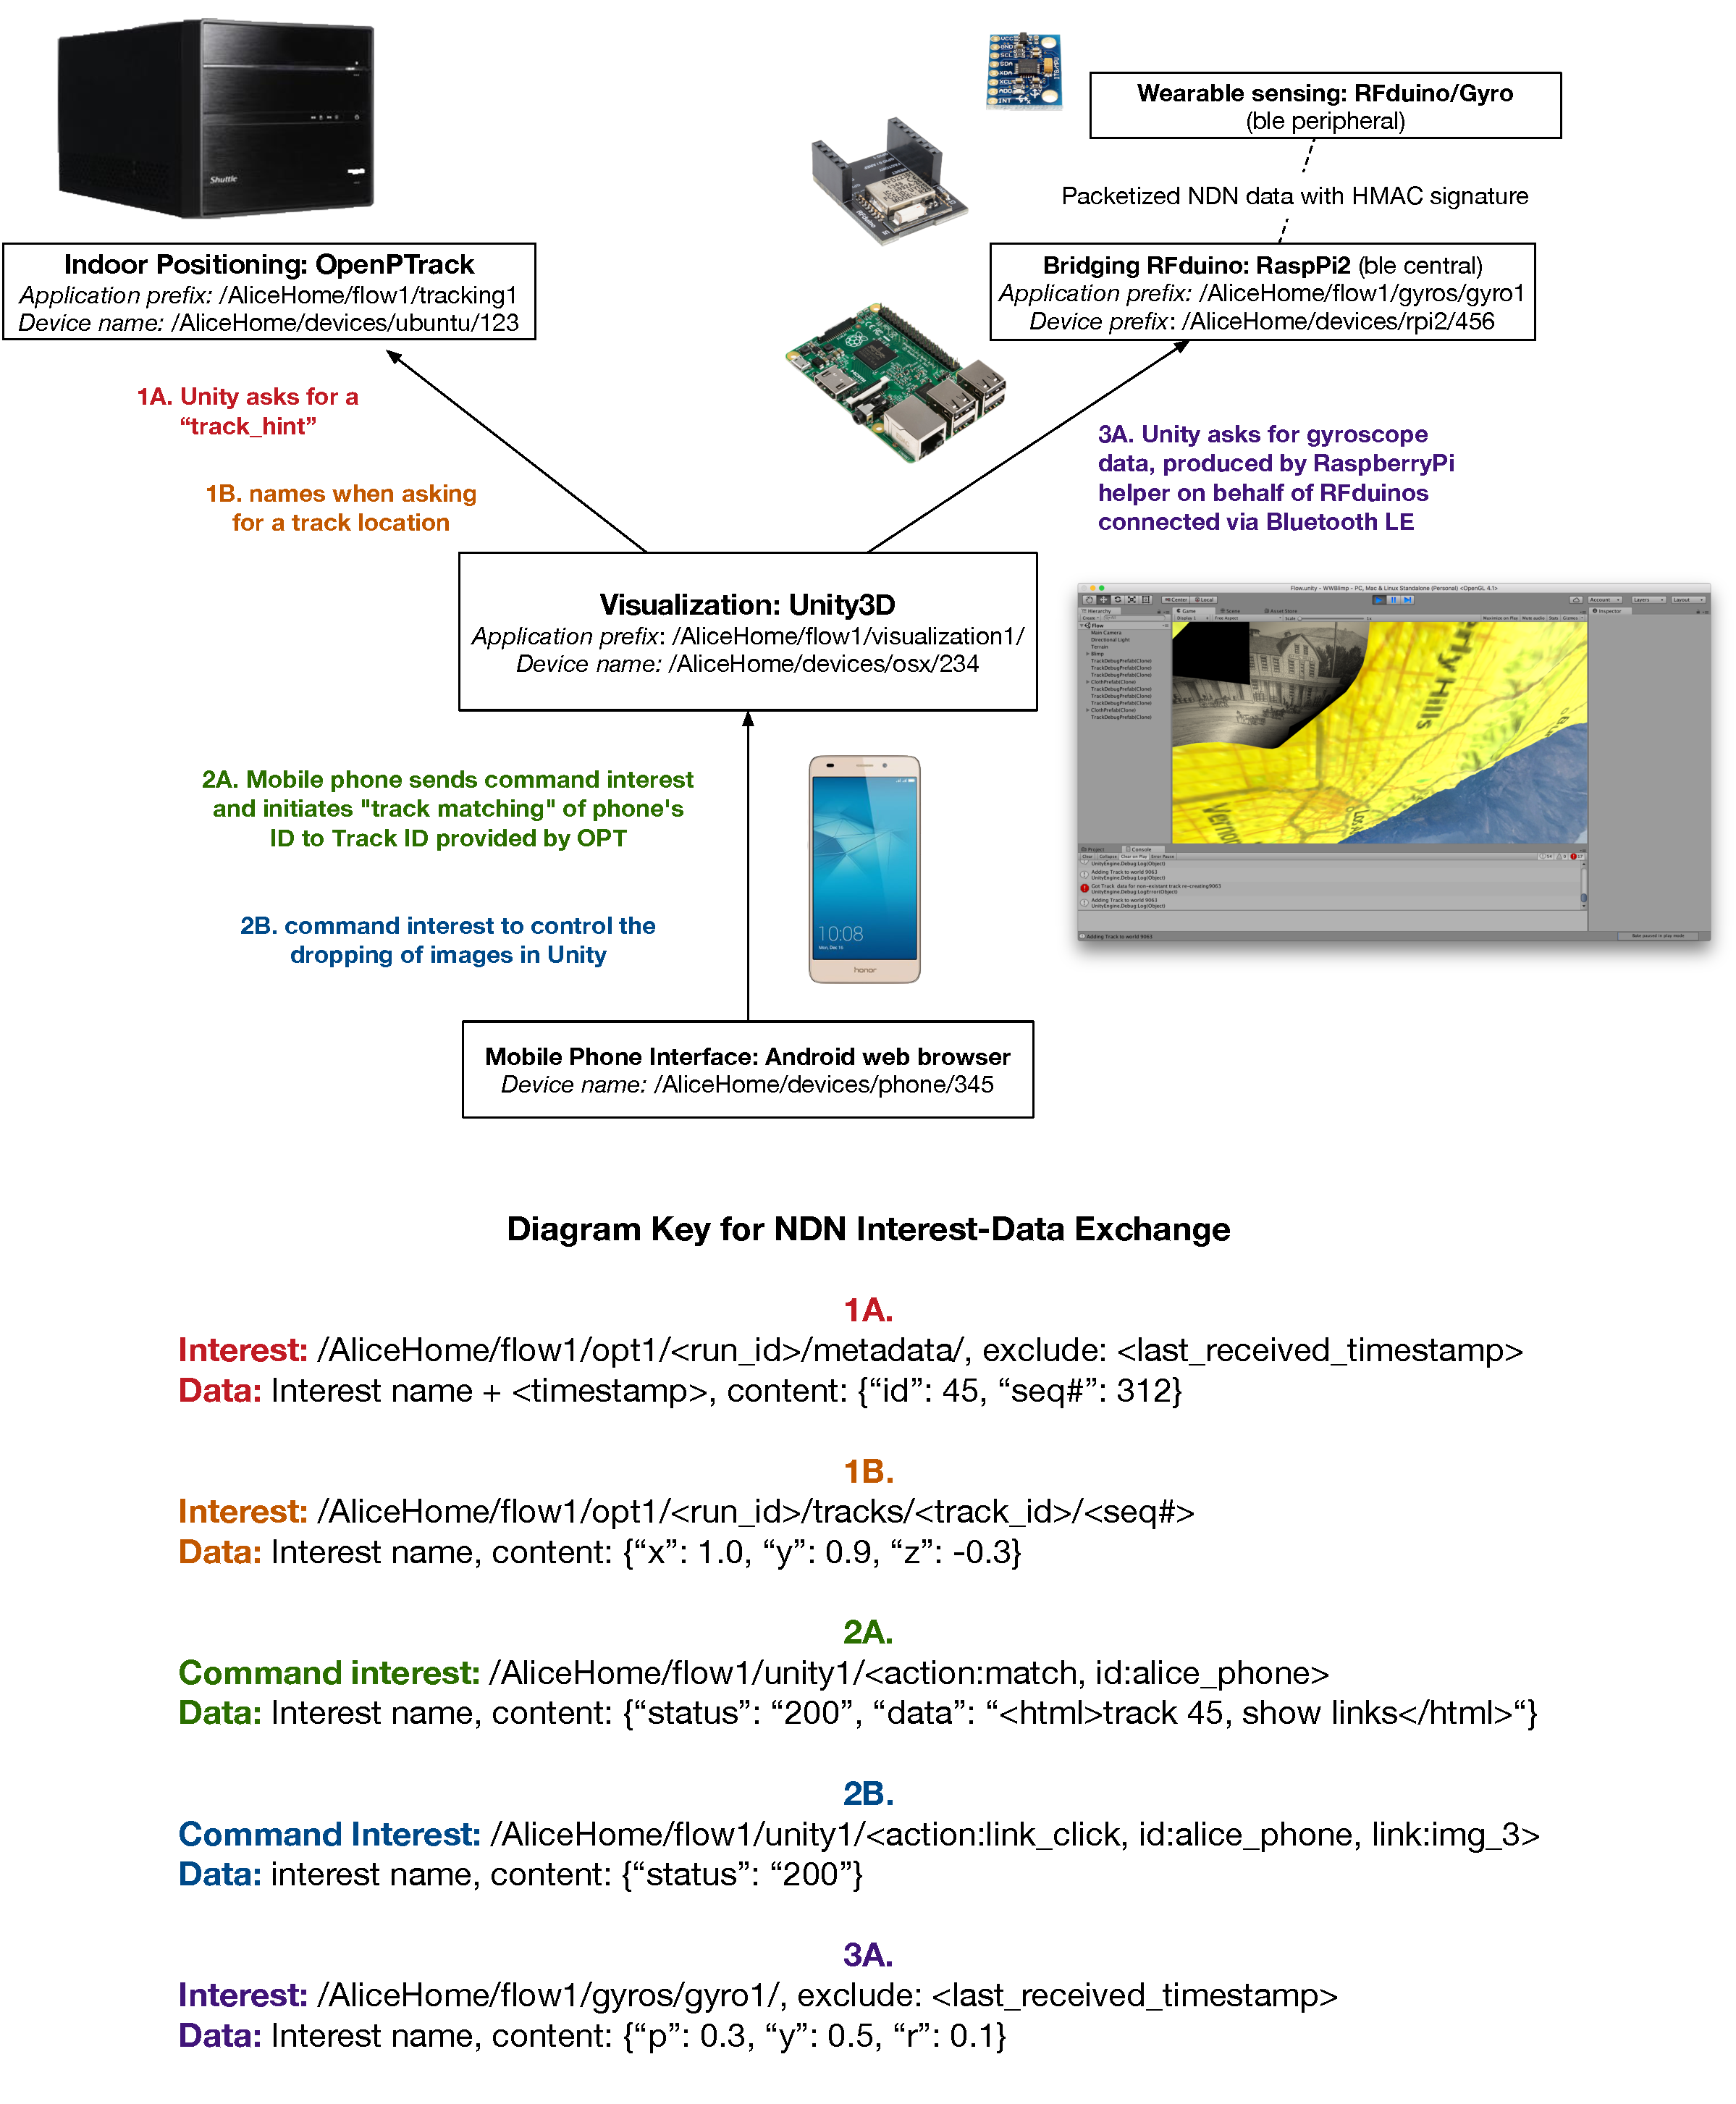
\includegraphics[width=0.95\textwidth]{flow-components-ndn-names-diagram-zs.pdf}
\caption{Application components and message flows in Flow}
\label{fig:message-flow-in-flow-installation}
\end{figure*}

For better visualization of data names in the system, we also implemented a namespace tree visualizer, which recursively expressed interest with previously received name components excluded, to probe data packets in the network.\footnote{The code is available at \url{https://github.com/zhehaowang/namespace-tree}. Since the installation of Flow it has been applied to other projects such as NDNFit and mini-BMS, and has gone through major UI revisions.}
% TODO: screenshot of namespace tree visualizer updated
% A screenshot of the namespace tree is shown in Figure~\ref{}

% \begin{figure*}[!t]
% \centering
% 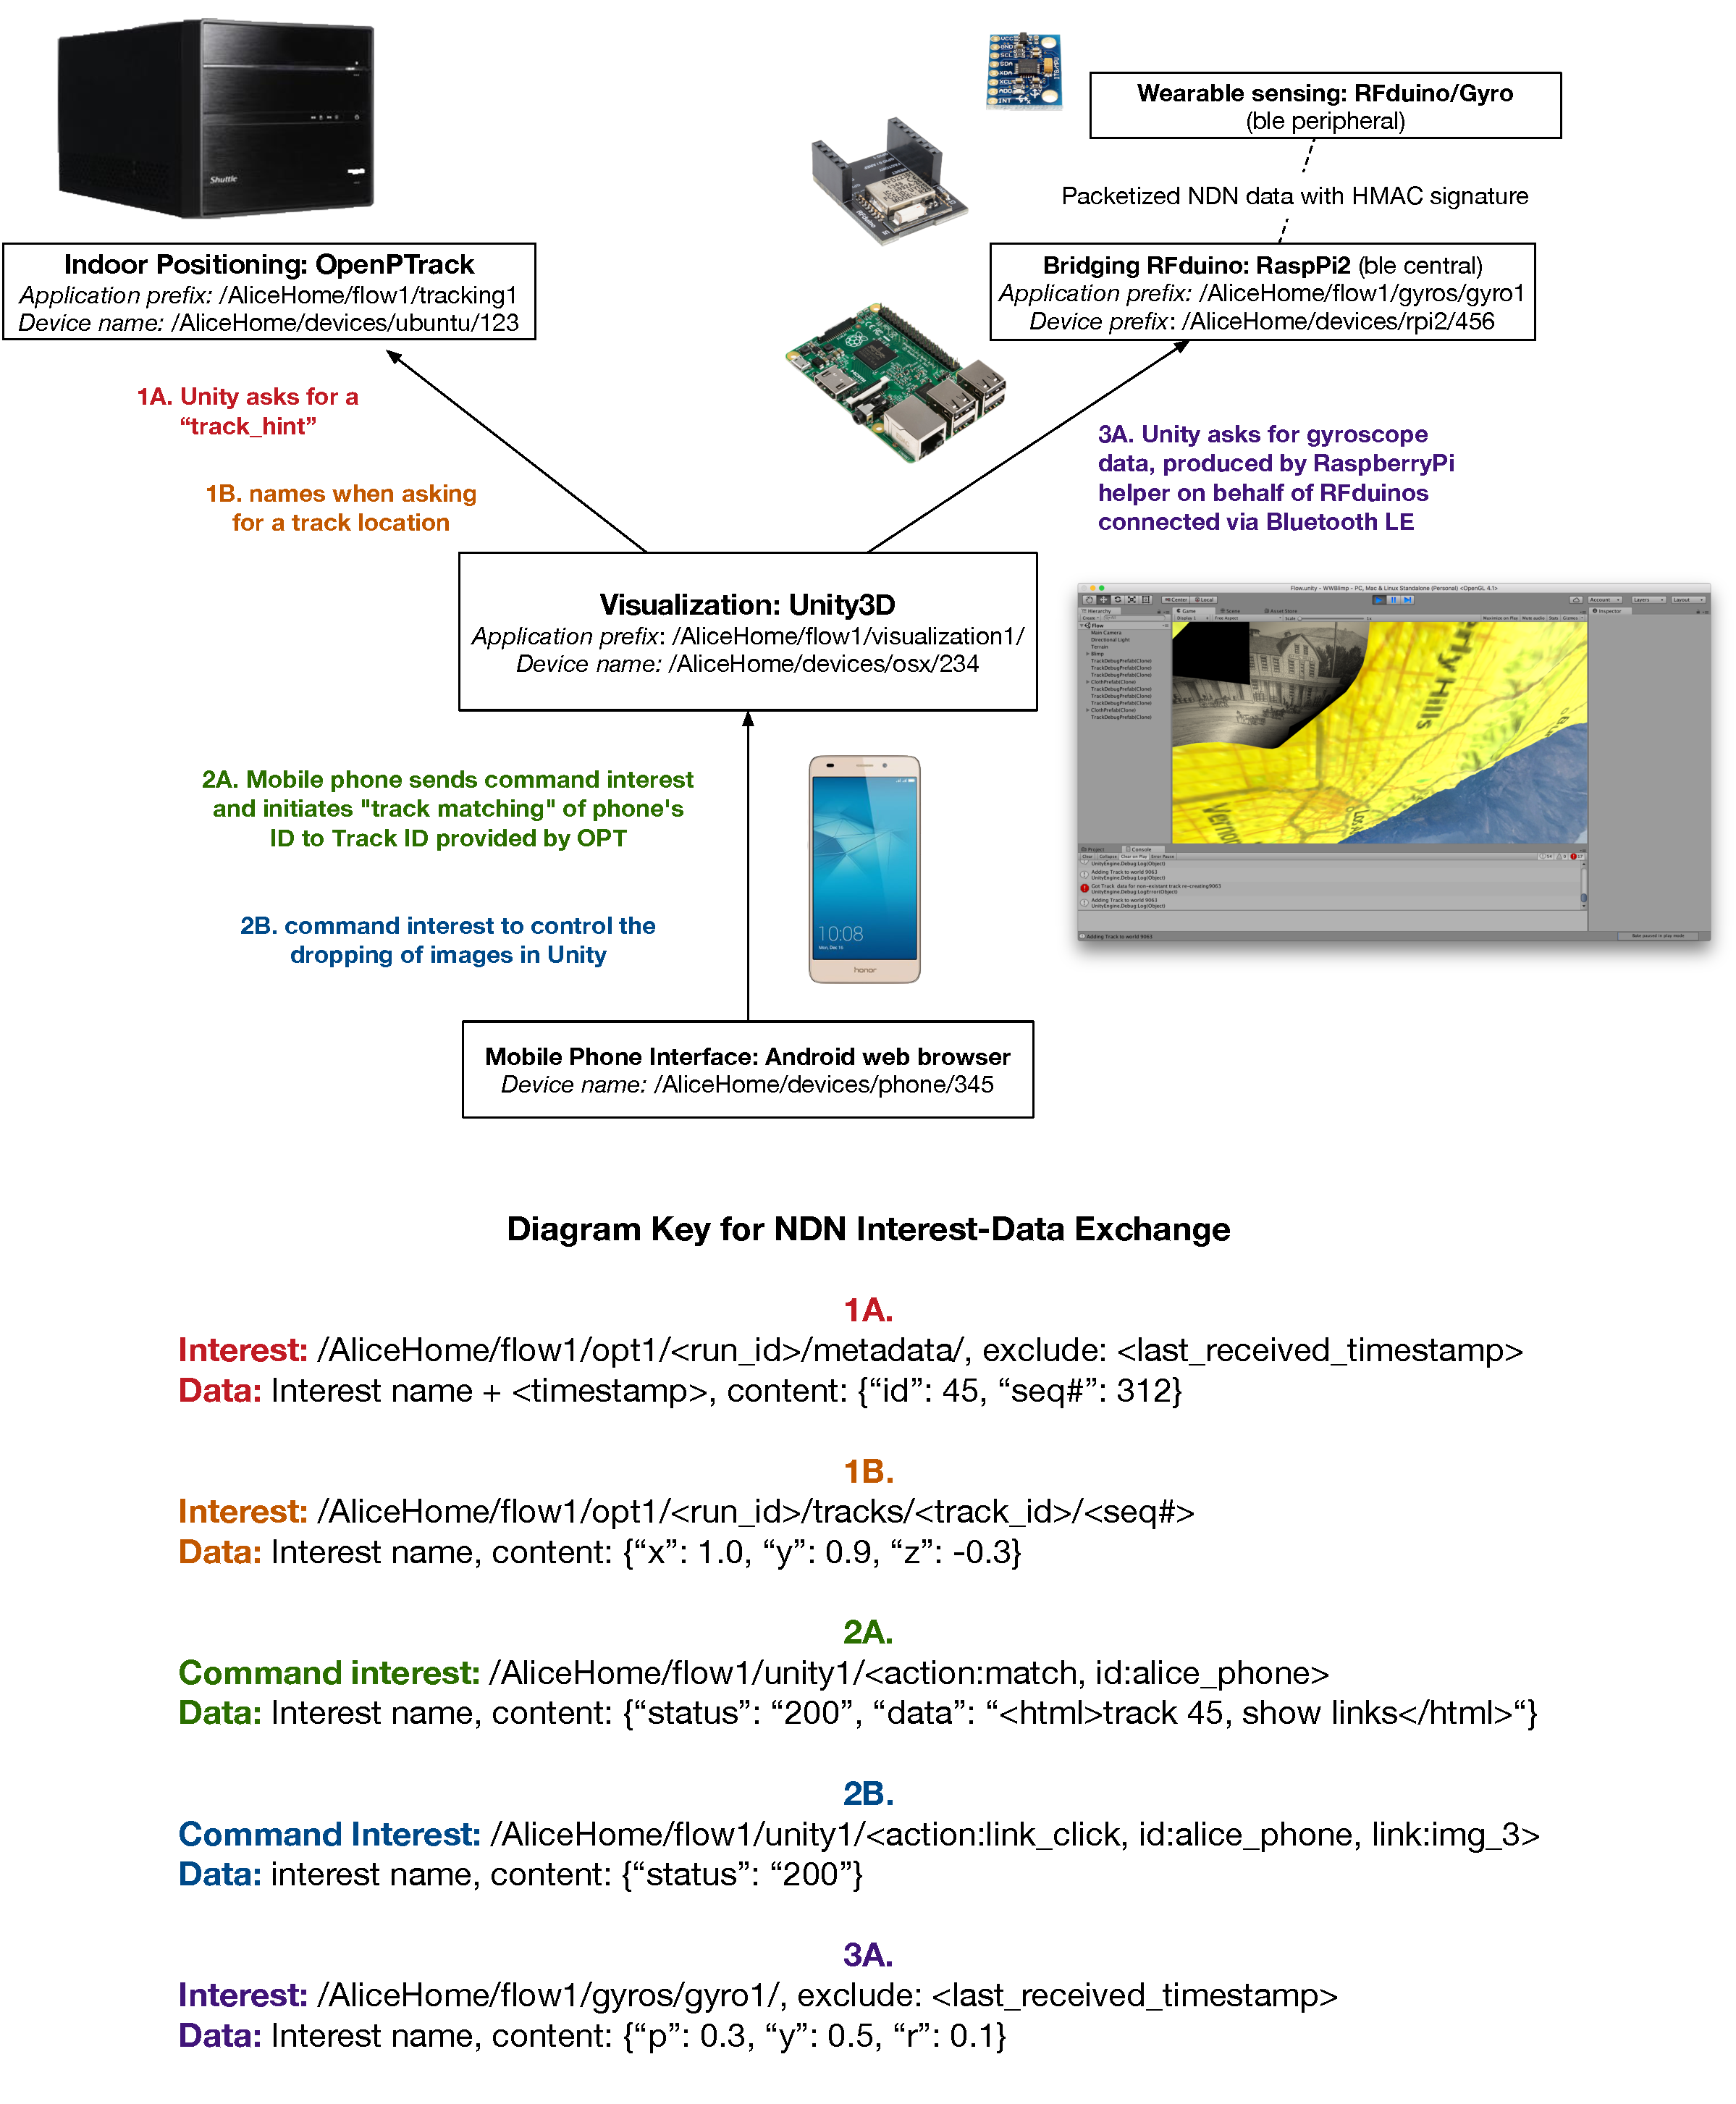
\includegraphics[width=0.95\textwidth]{flow-components-ndn-names-diagram-zs.pdf}
% \caption{Example namespace tree when running Flow application}
% \label{fig:namespace-tree}
% \end{figure*}